%THIS IS AN EXAMPLE OF HOW YOU MIGHT INTRODUCE A CHAPTER WHICH HAS ALREADY BEEN PUBLISHED.
\cleartoevenpage
\pagestyle{empty}	%Use this to suppress the header from the preceding chapter.

\noindent
The following published manuscript has been incorporated as Chapter~\ref{Chap:3}.

\noindent
\textbf{Wilkinson, Ross D.}, Andrew G. Cresswell, and Glen A. Lichtwark. 2020. Riders Use Their Body Mass to Amplify Crank Power during Nonseated Ergometer Cycling. \textit{Medicine $\&$ Science in Sports $\&$ Exercise}: Publish Ahead of Print. doi: 10.1249/MSS.0000000000002408

\begin{table}[h]
	\begin{center}
	\begin{tabular}{|c|l|l|}
		\hline
		Contributor & Statement of contribution & $\%$ \\
		\hline
		\textbf{Wilkinson, R.D.} & writing of text & 80\\
        & study design and concept & 20 \\
		& data collection & 90\\
        & data analysis & 90\\
		& statistical analysis & 100 \\
		& preparation of figures & 80 \\
		& revision of written work & 40 \\
		& supervision, guidance & 0 \\
		\hline
		Lichtwark, G.A. & writing of text & 10\\
        & study design and concept & 40 \\
		& data collection & 5 \\
        & data analysis & 5 \\
		& statistical analysis & 0 \\
		& preparation of figures & 10 \\
		& revision of written work & 30 \\
		& supervision, guidance & 50 \\
		\hline
		Cresswell, A.G. & writing of text & 10\\
        & study design and concept & 40 \\
		& data collection & 5 \\
        & data analysis & 5 \\
		& statistical analysis & 0 \\
		& preparation of figures & 10 \\
		& revision of written work & 30 \\
		& supervision, guidance & 50 \\
		\hline
	\end{tabular}
	\end{center}
\end{table}

%-------------------------------------------------------------------------------------------------------%
%-------------------------------------------------------------------------------------------------------%
%-------------------------------------------------------------------------------------------------------%
%-------------------------------------------------------------------------------------------------------%
%-------------------------------------------------------------------------------------------------------%
%-------------------------------------------------------------------------------------------------------%
%This is an internal chapter of the thesis.
%If you have a long title, you can supply an abbreviated version to print in the Table of Contents using the optional argument to the \chapter command.
\chapter[Riders Use Their Body Mass to Amplify Crank Power During Non-Seated Ergometer Cycling]{Riders Use Their Body Mass to Amplify Crank Power During Non-Seated Ergometer Cycling}
\label{Chap:4}	%CREATE YOUR OWN LABEL.
\pagestyle{headings}
%If you are presenting work which has been previously published, acknowledge this here.
%-------------------------------------------------------------------------------------------------------%
%-------------------------------------------------------------------------------------------------------%
%-------------------------------------------------------------------------------------------------------%
\section{Abstract}
When cyclists ride off the saddle, their centre of mass (CoM) appears to go through a rhythmic vertical oscillation during each crank cycle. Just like in walking and running, the pattern of CoM movement may have a significant impact on the mechanical power that needs to be generated and dissipated by muscle. \textbf{Purpose:} To date, neither the CoM movement strategies during non-seated cycling, nor the limb mechanics that allow this phenomenon to occur, have been quantified. \textbf{Methods:} Here we estimate how much power can be contributed by a rider's CoM at each instant during the crank cycle by combining a kinematic and kinetic approach to measure CoM movement and joint powers of fifteen participants riding in a non-seated posture at three individualised power outputs (10$\%$, 30$\%$, and 50$\%$ of peak maximal power) and two different cadences (70 rpm and 120 rpm). \textbf{Results:} The peak-to-peak amplitude of vertical CoM displacement increased significantly with power output and with decreasing cadence. Accordingly, the greatest peak-to-peak amplitude of CoM displacement (0.06 $\pm$ 0.01 m) and change in total mechanical energy (0.54 $\pm$ 0.12 J$\cdot$kg$^{-1}$) occurred under the combination of high-power output and low cadence. At the same combination of high-power output and low cadence, we found that the peak rate of CoM energy loss (3.87 $\pm$ 0.93 W$\cdot$kg$^{-1}$) was equal to 18$\%$ of the peak crank power. \textbf{Conclusion:} Consequently, it appears that for a given power output, changes in CoM energy contribute to peak instantaneous power output at the crank, thus reducing the required muscular contribution. These findings suggest that rise and fall of a rider's CoM acts as a mechanical amplifier during non-seated cycling, which has important implications for both rider and bicycle performance.

\section{Introduction}
When cyclists ride off the saddle during climbing and sprinting, their centre of mass (CoM) appears to go through a rhythmic vertical oscillation during each crank cycle. Early analyses of non-seated cycling from the late 1970's \autocite{Soden1978} and early 1990's \autocite{Hull1990} showed significant vertical oscillations of the rider's pelvis, providing indirect evidence that the CoM may follow a similar pattern. To date, no studies have quantified rider CoM movement, nor its impact on limb mechanics and crank power during non-seated cycling. Knowledge of CoM movement strategies during non-seated cycling is of importance as it may have a direct impact on the peak force and power that must be contributed by muscle during cycling, which in turn is a potential limiting factor to cycling performance. 

The movement pattern of an animal's CoM has a significant impact on the mechanical power that their muscles must generate or dissipate during locomotion \autocite{Cavagna1963,Cavagna1964}. For instance, when humans and many other terrestrial animals walk, run, or trot, they perform substantial amounts of mechanical work to redirect the CoM velocity during each step-to-step transition \autocite{Cavagna2017}. Although performing work to raise the CoM requires muscles to consume metabolic energy, this rise and fall of the CoM can save energy during locomotion through the storage and release of lost kinetic and potential energy as elastic strain energy in spring-like tendons \autocite{Alexander1991}. Likewise, we propose that when riding a bicycle off the saddle, vertical displacement of the CoM is important from both a mechanical and metabolic perspective. As evidenced during treadmill cycling, raising the CoM appears to benefit the rider by allowing a greater range of motion at the hip joint and is likely to alter the relative contribution of muscular and non-muscular sources to pedal force \autocite{Caldwell1998}. However, these benefits may be offset as raising the mass of the body against gravity requires additional energy to that which creates propulsion at the crank \autocite{VanIngenSchenau1990b}. Although net zero mechanical work is typically performed on the CoM over a complete crank cycle, at each instant within the crank cycle the interchange between gravitational potential energy and kinetic energy will dictate the total mechanical energy of the CoM; which in turn influences how much energy muscles need to generate and/or dissipate \autocite{Cavagna2017}. Determining the phasing and magnitude of changes in CoM mechanical energy may provide evidence that energy can be transferred between the CoM and the crank, which may reveal why riders choose to perform mechanical work to raise their CoM during non-seated cycling.

Previous research provides a strong indication that the gravitational and inertial components of pedal force are greater during non-seated compared to seated cycling \autocite{Stone1993, Caldwell1998}. Removing the saddle as a base of support means that a greater portion of bodyweight must be supported at the pedal \autocite{Caldwell1998}, while vertical motion of the pelvis suggests that the inertial contribution to pedal force is significantly higher than when seated \autocite{Soden1978, Hull1990}. Riders appear to utilise this non-muscular contribution to crank force by lowering their preferred cadence compared to when seated \autocite{Harnish2007,Lucia2001}. Furthermore, joint-level comparisons of seated and non-seated cycling at very high-power outputs suggest that the non-seated posture can increase the force-producing capabilities of the lower limb \autocite{Wilkinson2020a}. To date, the relative contribution of muscular and non-muscular sources to crank force and power during non-seated cycling have not been quantified.

Quantifying the contribution of non-muscular sources to crank force and power may help to explain why the non-seated posture is the most effective solution during certain sprinting and climbing scenarios. For example, in a group of highly trained cyclists (n=11, 4F/7M), maximal power output was 8$\%$ higher in a non-seated posture compared to seated (1567 vs. 1447 Watts) during a 5-s sprint at a cadence of 128 rpm on a level-ground ergometer \autocite{}(Hug et al. 2011). It has also been shown that during a 30-s Wingate test against a fixed resistance, competitive college cyclists (n=12) produced a mean power output of 11.0 $\pm$ 0.4 W$\cdot$kg$^{-1}$ at a cadence of 127 $\pm$ 5 rpm when non-seated compared to 10.4 $\pm$ 0.6 W$\cdot$kg$^{-1}$ at a cadence of 121 $\pm$ 6 rpm when seated \autocite{ReiserII2002}. Furthermore, the non-seated posture appears to significantly increase time to exhaustion during treadmill cycling on a 10$\%$ incline at power outputs approaching 9.6 $\pm$ 0.7 W$\cdot$kg$^{-1}$ \autocite{Hansen2008}. Further biomechanical analyses are required to shed light on the mechanisms that underpin the increase in sprinting and climbing performance when non-seated compared to seated. 

Here we combined a kinematic and kinetic approach to measure CoM movement and joint power of fifteen participants riding in a non-seated posture at a range of individualised but controlled power outputs (10$\%$, 30$\%$, and 50$\%$ of instantaneous maximal power output (\textit{P}$_{max.i}$) at two different cadences (70 rpm and 120 rpm). Our first prediction was that additional power to that measured at the crank would be generated by the rider to raise the CoM during the crank cycle. Secondly, the phasing and magnitude of CoM motion would change with power output and cadence due to the different magnitude, direction, and duration of forces, and thirdly that the potential energy gained by raising the CoM would be used to amplify positive crank power; making raising and lowering of the CoM potentially useful.

\section{Materials and methods}
\subsection{Experimental design}
We tested 15 men (age 30 $\pm$ 8 years, height 1.79 $\pm$ 0.05 m, and mass 74.4 $\pm$ 8.5 kg); eight of whom were cyclists who competed we\textit{E}$_{k}$ly at club level, while the others regularly engaged in a variety of competitive or recreational sports. The recruitment of roughly equal numbers of cyclists and non-cyclists was not intentional nor a focus of the study. Post-hoc analysis confirmed that cycling experience did not significantly affect instantaneous maximal power output capability between the two groups (cyclists=22.6 $\pm$ 5 W$\cdot$kg$^{-1}$ vs. others=20.6 W$\cdot$kg$^{-1}$, $\rho$=0.35). All participants gave their written informed consent prior to participating in this study according to the procedures approved by the Human Ethics Committee of The University of Queensland and in accordance with the general principles expressed in the Declaration of Helsinki. For the regular cyclists, we matched the seat height and handlebar position of the ergometer (Excalibur Sport, Lode BV, Groningen, The Netherlands) to their accustomed cycling position. For the remaining participants, we standardized fitting to an internal knee angle of 150\textdegree and torso angle (trunk relative to horizontal) of 70\textdegree. Based on each cyclist's preference, we made minor adjustments to this fitting. Crank length was set to 175 mm. Participants wore cleated cycling shoes (SH-R070, Shimano, Osaka, Japan) that clipped into the pedals (SH-R540, Shimano, Osaka, Japan).

The test session began with a 5-min cycling warm-up at 100 W at their preferred cadence. To individualise power output in the sub-maximal trials we first determined each participant's instantaneous maximal power output (\textit{P}$_{max.i}$) by having them perform five maximal sprints of 3 s duration in a seated posture. We calculated \textit{P}$_{max.i}$ as the highest ``instantaneous'' power that occurred during a crank cycle. The ergometer was set to ``Linear'' mode, which ensured the coupling of power output and cadence. Participants were given a familiarization trial before performing the test. For all sprints, the participant began with the crank and flywheel stationary. The initial resistance was based on \textit{P}$_{max.i}$ results from pilot testing three individuals. We expected that participants would achieve \textit{P}$_{max.i}$ at a cadence close to 120 rpm \autocite{Dorel2018a}. Thus, we increased or decreased the linear resistance of the ergometer for the subsequent trial based on whether the participant achieved a cadence above or below 120 rpm. A 3-min rest period was given between trials to reduce any potential fatigue effects. For all participants, it took five or less sprint trials to determine the resistance which elicited their \textit{P}$_{max.i}$. 

A rest period of 20-min was given after the \textit{P}$_{max.i}$ test before beginning the six sub-maximal trials. Participants performed combinations of power output (10$\%$, 30$\%$, and 50$\%$ of \textit{P}$_{max.i}$) and cadence (70 rpm and 120 rpm) in a randomized order. Participants were required to maintain the target cadence and power output for a minimum period of 10 s. The ergometer was set to ‘Hyperbolic' mode, which ensured that power output remained constant independent of cadence. Thus, participants were required to maintain the target cadence using feedback from the visual display on the ergometer. Post-hoc analyses confirmed that the target cadences were met across all trials in each cadence condition (70 rpm=71.9 $\pm$ 0.5 rpm, 120 rpm=120.7 $\pm$ 2.0 rpm). Following the sub-maximal trials, the presence of exercise-induced fatigue was assessed by asking each participant to perform an additional 3-s maximal sprint. Inclusion required the participant to match, within $\pm$ 5$\%$, their previously tested \textit{P}$_{max.i}$ in this added maximal sprint. For each sub-maximal trial, we acquired crank angle and force signals synchronously with motion capture using a 16-bit A/D conversion board (USB-2533, Measurement Computing Corporation, Norton, MA) and Qualisys Track Manager Software (Qualisys AB, Gothenburg, Sweden).

\subsection{Kinematics}
The three-dimensional (3D) positions of 45 passive reflective markers were collected at 200 Hz using an eight camera, opto-electronic motion capture system (Oqus, Qualisys, AB, Sweden). Reflective markers were secured to the skin using double-sided tape over the suprasternal notch, C7 spinous process, sacrum, and bilaterally over the acromion processes, lateral epicondyles of the humerus, styloid processes of the radius, iliac crests, anterior superior iliac spines, posterior superior iliac spines, greater trochanters, medial and lateral condyles of the femur, and medial and lateral malleoli. Markers were secured to the cycling shoe over the calcanei, heads of the 1st and 5th metatarsals and the 2nd distal phalanxes. Lightweight, rigid clusters of four markers were also secured bilaterally to the lateral mid-thighs and lateral mid-shanks using double-sided tape and self-adhesive bandage. A static trial was collected with the participant standing in a standard anatomical posture before commencing the sub-maximal trials. This trial was used for kinematic model scaling. The heading (yaw) angle of the ergometer was determined within the motion capture global coordinate system by placing two markers on the rear support legs of the ergometer. These markers were used to create a local coordinate system for the ergometer, which accounted for any discrepancy with the global coordinate system between trials.

\subsection{External forces}
We recorded tangential and radial forces at the left and right crank, as well as crank angle at 100 Hz using pre-calibrated, wireless, instrumented cranks (Axis, SWIFT Performance, Brisbane, Australia). Digital signals were transmitted wirelessly to a base receiver before being converted to an analogue signal through the A/D Board. The internal sampling factor within Qualisys Track Manager Software matched the digital sampling frequencies of the crank (100 Hz) to the motion capture (200 Hz) sampling frequency. Each crank was independently calibrated by performing a multi-axis, dynamic calibration. In addition, and prior to testing, we calibrated the output voltage for the tangential and radial force by suspending a 2.5 kg mass from each pedal spindle with the cranks in both horizontal and vertical positions. A spirit level was used to zero the crank angle of the right crank at top dead centre (TDC).

Equations \ref{eq:Fz2} and \ref{eq:Fhb2} show how the net force acting at the handlebar (F$_{hb}$) was calculated by comparing the total vertical force (F$_z$) required to cause the measured accelerations of the rider's CoM (a$_{com}$) with the sum of vertical force at the left (F$_{cl}$) and right (F$_{cr}$) cranks. The remainder is an estimate of the net vertical force acting on the hands of the rider at the handlebar (F$_{hb}$). Thus, a net positive vertical handlebar force pertains to the reaction force induced by a net downward pushing force from the arms/body and a negative vertical reaction force pertains to a net upward pulling force from the arms/body. A limitation to the calculation of net F$_{hb}$ is that it cannot identify whether simultaneous pushing and pulling forces are being generated. A diagram of the net vertical forces acting on the rider are displayed in Figure \ref{fig:m2f0}A.

\begin{equation}
    F_z = m \cdot (g + a_{com})
    \label{eq:Fz2}
\end{equation}
\begin{equation}
	F_{hb} = F_z - (F_{cr} + F_{cl})	  
	\label{eq:Fhb2}
\end{equation}

\subsection{Mechanical energy and power}

Motion capture marker trajectories, crank forces, and crank angles were processed using custom scripts in MatLab (R2018b, Mathworks Inc., USA). These scripts filtered crank force signals and marker trajectories with a zero-lag, second-order, low-pass Butterworth filter with a cut-off frequency of 12 Hz \autocite{Kristianslund2012}. The measured angular position of the crank was rotated into the global coordinate system to transform the respective crank forces (tangential and radial) into their horizontal and vertical components. The force components and marker trajectories were then rotated into the ergometer coordinate system. The origin of the resultant force was determined by creating a virtual marker at the centre of the cleat. This approximation was determined using the crank angle, three-dimensional shoe orientation, and shoe size. We then verified this first approximation against a second approximation using the bottom bracket position, crank length, crank angle, and pedal spindle length.

OpenSim software \autocite{Delp2007} was used to create participant-specific models by scaling segment lengths and segment masses of a previously developed generic full-body musculoskeletal model \autocite{Rajagopal2016} based on each participant's anthropometry. Inverse kinematic analysis was used to calculate joint kinematics \autocite{Seth2011}. Inverse dynamic analysis was used to calculate hip, knee, and ankle net joint moments by combining the inverse kinematics results with external loads applied to the model, in this case reaction forces at the left and right crank \autocite{Seth2011}. Joint power was calculated as the dot product of the net joint moment and joint angular velocity. Flexor moments and flexion velocity were defined as positive and joint work as the integral of joint power with respect to time. Inclusion of data required the cyclist to simultaneously match the target power ($\pm$ 5$\%$) and cadence ($\pm$ 5$\%$) at the right crank for a minimum of five consecutive crank cycles.

In cycling, positive power generated by muscle is dissipated to the environment (excluding gravity), conservative forces (including gravity and the stretching of elastic elements), and non-conservative forces such as friction and drag \autocite{VanIngenSchenau1990b}. More specifically, the rider imparts motion to the rider-bicycle system by overcoming aerodynamic drag, rolling resistance, wheel bearing friction, the rate of change of potential and kinetic energy, and friction in the drive train \autocite{Martin1998}. Typically, it is assumed that the rider's CoM travels parallel to the riding surface, meaning that the change in potential and kinetic energy of the rider's CoM is reflected by the change in the potential and kinetic energy of the system. Under this assumption power measured at the cranks will be equivalent to the total power output generated by the rider. However, this assumption does not account for any movement of the rider's CoM relative to the reference frame of the bicycle. Evidence suggests that this is particularly important when cycling in a non-seated posture, where it appears that the rider's CoM is raised and lowered periodically during the crank cycle \autocite{Soden1978,Hull1990}. Thus, the total joint power generated by the rider (\textit{P}$_{tot}$) at each instant during the crank cycle will be equivalent to power measured at the cranks (\textit{P}$_{cranks}$) plus energy lost or gained by the rider's CoM with respect to time (\textit{P}$_{CoM}$) as shown in Equation \ref{eq:Ptot2}.

\begin{equation}
    P_{tot} = P_{cranks} + P_{CoM}
    \label{eq:Ptot2}
\end{equation}

\begin{equation}
    P_{lb} + P_{ub} = P_{cranks} + P_{CoM}
    \label{eq:Plb2}
\end{equation}

In this study, \textit{P}$_{cranks}$ was calculated as the summed dot product of torque and angular velocity measured at each crank. \textit{P}$_{CoM}$ was calculated using the inverse kinematic results as the sum of the change in potential energy (\textit{E}$_\textit{P}$) and kinetic energy (\textit{E}$_k$) of each segment divided by the change in time. Kinetic energy of motion (a scalar quantity) was accounted for in all axes by using the square of the resultant velocity of the CoM in x, y, and z axes multiplied by half mass. Kinetic energy due to angular motion of the CoM was deemed negligible. \textit{P}$_{tot}$ can also be thought of as the sum of lower body and upper body joint power as shown in Equation \ref{eq:Plb2}. Lower body joint power (\textit{P}$_{lb}$) was calculated using inverse dynamic results as the summed dot product of net joint moments and joint angular velocities at the hip, knee, and ankle of each leg. Upper body power (\textit{P}$_{ub}$) was assumed to be the difference between \textit{P}$_{tot}$ and \textit{P}$_{lb}$, which can be attributed to the net power generated by muscles crossing the joints within the arms and trunk. A limitation of this calculation of \textit{P}$_{ub}$ is that it cannot identify whether power is being simultaneously generated and dissipated within the upper body. To illustrate these calculations, a plot of \textit{P}$_{tot}$ with respect to crank angle is shown in Figure \ref{fig:m2f0}B split into its components of \textit{P}$_{cranks}$ and \textit{P}$_{CoM}$ and its components of \textit{P}$_{lb}$ and \textit{P}$_{ub}$ (right).

\begin{figure}[htbp]
    \centering
    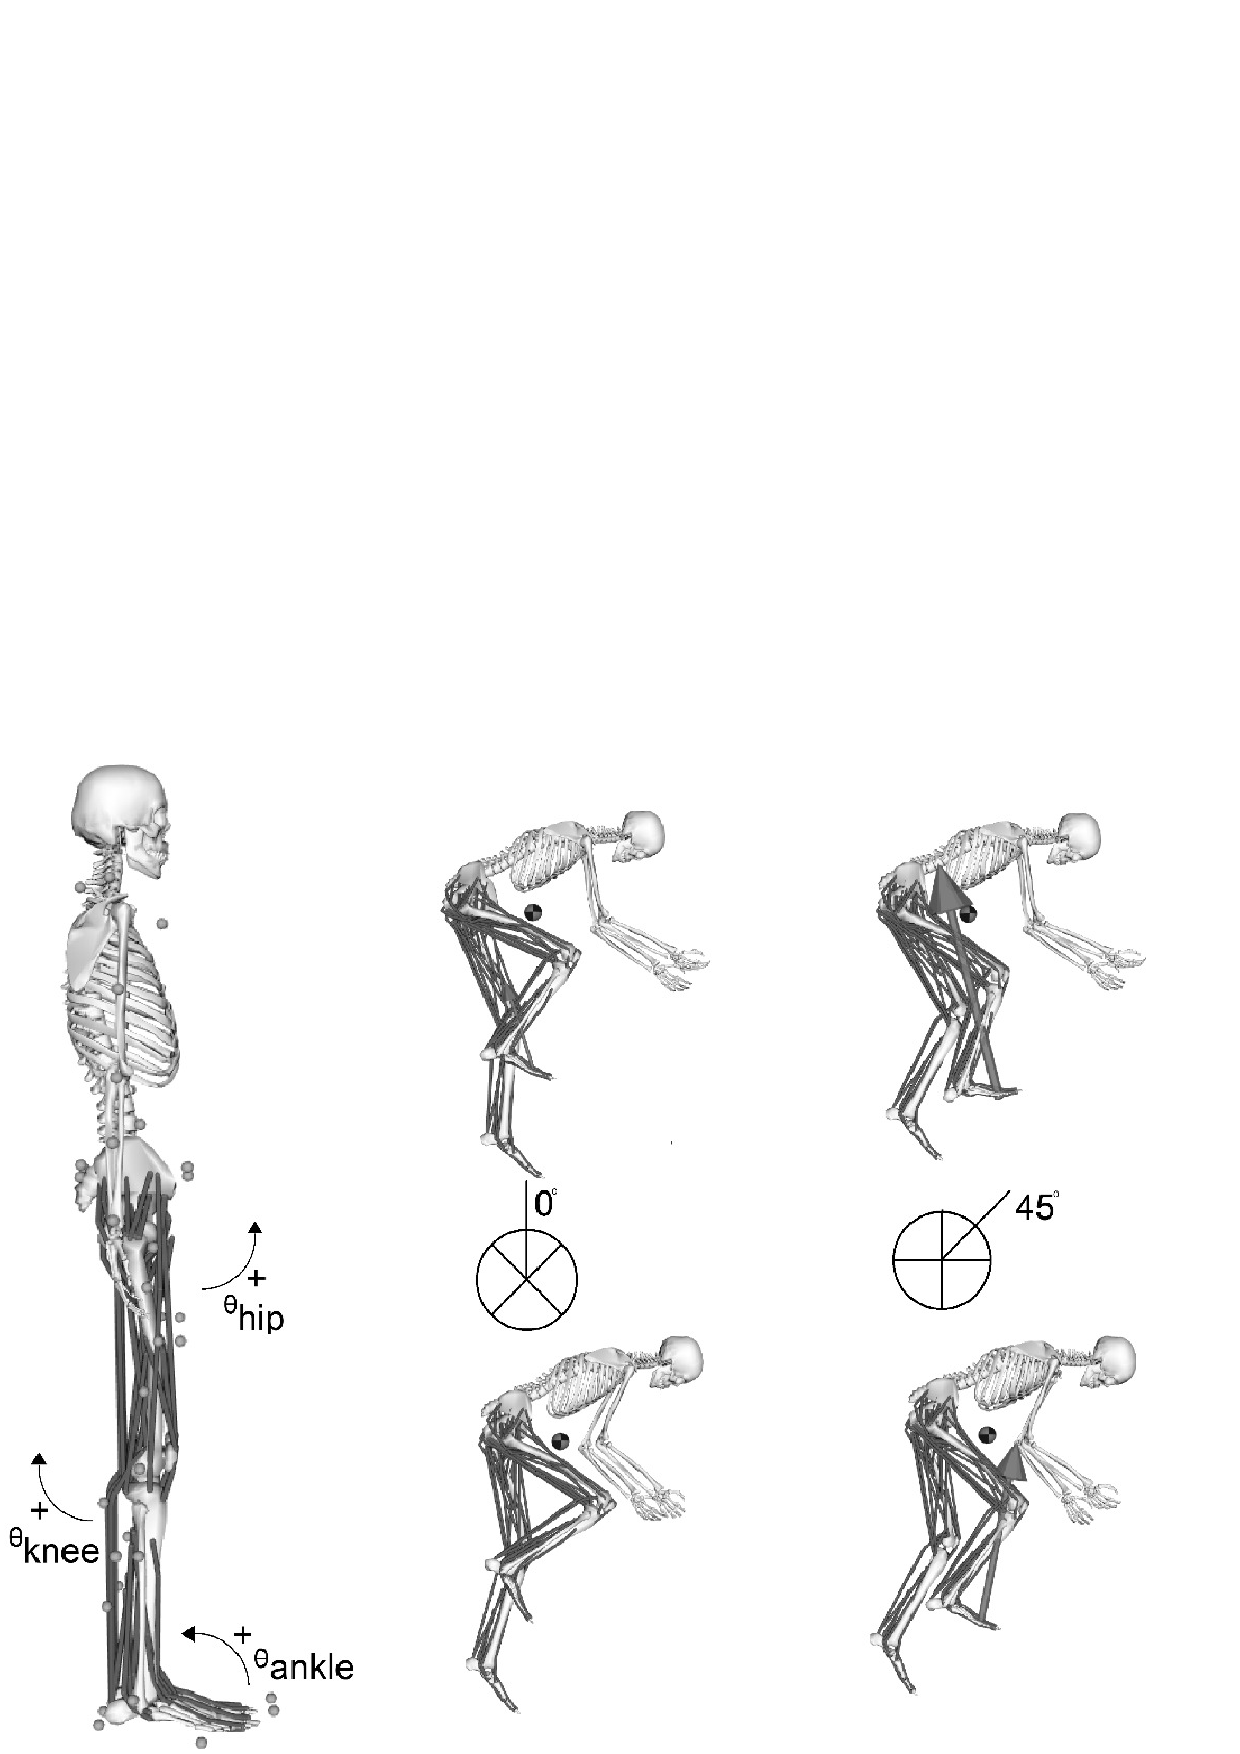
\includegraphics[width=\textwidth]{Study2/Figure1.png}
    \caption[Calculations of instantaneous total joint power must account for any change in gravitational potential energy and kinetic energy of the rider's CoM relative to the reference frame of the bicycle.]{\textbf{Calculations of instantaneous total joint power must account for any change in gravitational potential energy and kinetic energy of the rider's CoM relative to the reference frame of the bicycle.} A. Diagram of vertical forces acting on the rider during non-seated cycling. The measured vertical accelerations of the rider's CoM must be in equilibrium with the sum of vertical interaction force between the rider and the bicycle. F$_{va}$ represents the net vertical force that must be counteracted to cause the measured acceleration of the rider's CoM; F$_{vcr}$ and F$_{vcl}$ are, respectively, the measured vertical components of the reaction force impressed by each foot on the right and left crank, and F$_{vhb}$ is the vertical component of the net reaction force at the handlebar, calculated as the difference between F$_{va}$ and the sum of F$_{vcr}$ and F$_{vcl}$. B. Total joint power generated by the rider normalised to body mass (\textit{P}$_{tot}$) separated into the measured power at the left and right crank (\textit{P}$_{cranks}$) and the rate of energy gained and lost by the rider's CoM (\textit{P}$_{CoM}$). C. Total joint power generated by the rider (\textit{P}$_{tot}$) separated into the calculated power in the left and right lower limb (\textit{P}$_{lb}$) and the net power generated on, and by, the upper body (\textit{P}$_{ub}$). Data shown is the mean $\pm$ one standard deviation (shaded area) of one subject over 15 crank cycles during non-seated cycling at 30$\%$ \textit{P}$_{max.i}$ (8.5 W$\cdot$kg$^{-1}$) and 70 rpm.}
    \label{fig:m2f0}
\end{figure}

\subsection{Statistical analyses}
We performed repeated measures, two-way analyses of variance (ANOVAs) to test for main effects of power and cadence and interaction effects (power x cadence) on the peak-to-peak amplitude of CoM displacement and energy, peak CoM power, net lower body power, and net upper body power. The alpha level for main and interaction effects was set at 0.037 prior to statistical analysis. This alpha level was based on a desired false positive risk of <5$\%$, a prior probability for a real effect of 0.5, sample size of fifteen, and an estimated effect size of 1 \autocite{FPRcalc}. Whenever a main or interaction effect was found, multiple comparisons were used to detect the effect of the factor/s in each condition. The alpha level was corrected for familywise multiple comparisons using the Sidak method. The F-value (\textit{F}), p-value ($\rho$), and generalized eta squared ($\eta^2_G$) are provided for main and interaction effects. For multiple comparisons the t-statistic (t), adjusted p-value ($\rho$), 95$\%$ confidence intervals (95$\%$CI [Low-High]), and corrected effect size, known as Hedge's g$_{av}$ (ES), are provided. The $\eta^2_G$ for each variable was assessed against the benchmarks of trivial (<0.0099), small (0.0099-0.0588), moderate (0.0588-0.1379), and large effect (>0.1379) \autocite{Lakens2013}. The ES for each variable was assessed against the commonly used benchmarks of small (0.1-0.3), moderate (0.3-0.5) and large effect (>0.5). All values are reported as mean $\pm$ standard deviation.

\FloatBarrier

\section{Results}
We first sought to quantify rider CoM kinematics and associated mechanical energy changes during non-seated cycling under six combinations of power output and cadence.  The group mean CoM displacement in 3D space highlighted that CoM displacement occurred predominantly in the vertical (Z) axis (See Figure, Appendix \ref{fig:m2f2}, which shows 3D plots of CoM displacement in each condition). The peak-to-peak amplitude of CoM displacement, velocity, and acceleration increased significantly with increasing power output at each cadence (See Figure, Appendix \ref{fig:m2f2}, which shows CoM displacement, velocity, and acceleration with respect to crank angle in each condition). Figure \ref{fig:m2f3} shows the group mean change in potential, kinetic, and total CoM mechanical energy with respect to crank angle for each condition.

In support of our first hypothesis, substantial increases in potential energy of the CoM occurred predominantly in the first half of each leg's down-stroke (0-90\textdegree) without an equal decrease in kinetic energy, confirming that work performed by muscle was required to raise the rider's CoM. Likewise, substantial decreases in potential energy occurred during the second half of each leg's downstroke (90-180\textdegree) without an equivalent decrease in kinetic energy, meaning energy of the CoM was most likely transferred to the crank. Importantly, the timing of CoM energy changes with respect to crank angle showed that the CoM was raised from its lowest height to its peak height using predominantly forces that did not impede crank power (i.e. radial forces), while the lowering of the CoM occurred when the rider's mass could most effectively contribute to tangential force, and hence power at the crank.

The group mean maximal peak power output was 1605 $\pm$ 368 W (21.5 $\pm$ 4 W$\cdot$kg$^{-1}$), meaning that the individualised power outputs of 10$\%$, 30$\%$, and 50$\%$ of \textit{P}$_{max.i}$ corresponded to 2.1 $\pm$ 0.4, 6.4 $\pm$ 1.2 and 10.7 $\pm$ 2.0 W$\cdot$kg$^{-1}$, respectively. At each power output, regular oscillations of the total CoM mechanical energy (\textit{E}$_{tot}$) occurred within each crank cycle, with only minor in-phase and out-of-phase exchanges of kinetic energy (\textit{E}$_{k}$) and gravitational potential energy (\textit{E}$_{p}$) (See Figure \ref{fig:m2f3}). Maximum and minimum \textit{E}$_{tot}$ occurred earlier in the crank cycle at the lower cadence and shifted progressively earlier as power output increased for both cadence conditions. \textit{E}$_{tot}$ reached a single maximum value during the power phase for each leg (i.e. twice per 360\textdegree cycle of the right crank as seen in Figure \ref{fig:m2f3}). After reaching peak height at a crank angle of approximately 45\textdegree, the CoM lowered to a minimum height at a crank angle of approximately 135\textdegree. Thus, it is possible that the majority of energy lost by the CoM (\textit{E}$_{tot}$) during this phase contributed to positive work at the crank. Peak downward velocity of the CoM occurred between crank angles of 90\textdegree and 135\textdegree (See Figure, Appendix \ref{fig:m2f2}) and were coincident with vertical forces being equal to bodyweight (F$_{va}$) (See Figure \ref{fig:m2f3}). Vertical forces greater than bodyweight acted to decrease the downward velocity of the CoM during the later stages of the downstroke and then to accelerate the CoM back to a maximum height ready for the power phase of the opposite leg. In all conditions, the downstroke leg ($\sim$135-225\textdegree) produced the majority of vertical force to raise the CoM from its lowest position to its highest (60 $\pm$ 9$\%$), followed by the handlebars (25 $\pm$ 6$\%$), and the opposite leg ($\sim$315-45 \textdegree) (16 $\pm$ 4$\%$). A greater portion of bodyweight was supported at the handlebar across the crank cycle at 120 rpm (10$\%$ \textit{P}$_{max.i}$=36 $\pm$ 8$\%$, 30$\%$ \textit{P}$_{max.i}$ =29 $\pm$ 16$\%$, 50$\%$ \textit{P}$_{max.i}$ =20 $\pm$ 26$\%$) compared to 70 rpm (10$\%$ \textit{P}$_{max.i}$=32 $\pm$ 9$\%$, 30$\%$ \textit{P}$_{max.i}$ =16 $\pm$ 19$\%$, 50$\%$ \textit{P}$_{max.i}$ =1 $\pm$ 28$\%$) at each power output. At both cadences, the portion of bodyweight supported at the handlebar decreased as power output increased. 

In support of our second hypothesis, increasing power output and lowering cadence each increased the peak-to-peak amplitude of rider CoM displacement. Statistical analyses showed large main effects of power output (\textit{F}=21, $\rho$=<0.001, $\eta^2_G$=0.25) and cadence (\textit{F}=268, $\rho$=<0.001, $\eta^2_G$=0.73) and a moderate interaction effect (\textit{F}=8.1, $\rho$=0.002, $\eta^2_G$=0.06) on the peak-to-peak amplitude of CoM displacement. The peak-to-peak amplitude of changes in \textit{E}$_{tot}$ increased significantly with power output at 70 rpm (10$\%$=0.34$\pm$0.10, 30$\%$=0.44$\pm$0.09, and 50$\%$=0.54$\pm$0.12 J$\cdot$kg$^{-1}$) and at 120 rpm (10$\%$=0.12$\pm$0.04, 30$\%$=0.14$\pm$0.06, and 50$\%$=0.22$\pm$0.10 J$\cdot$kg$^{-1}$) and were significantly greater at 70 rpm than at 120 rpm at each power output (See Figure \ref{fig:m2f3}). Although not tested statistically, the peak-to-peak amplitude of changes in \textit{E}$_{tot}$ appears to increase roughly linearly with power output under both cadence conditions, but the rate of increase is seemingly greater at low cadence compared to high cadence.

\begin{figure}[htbp]
    \centering
    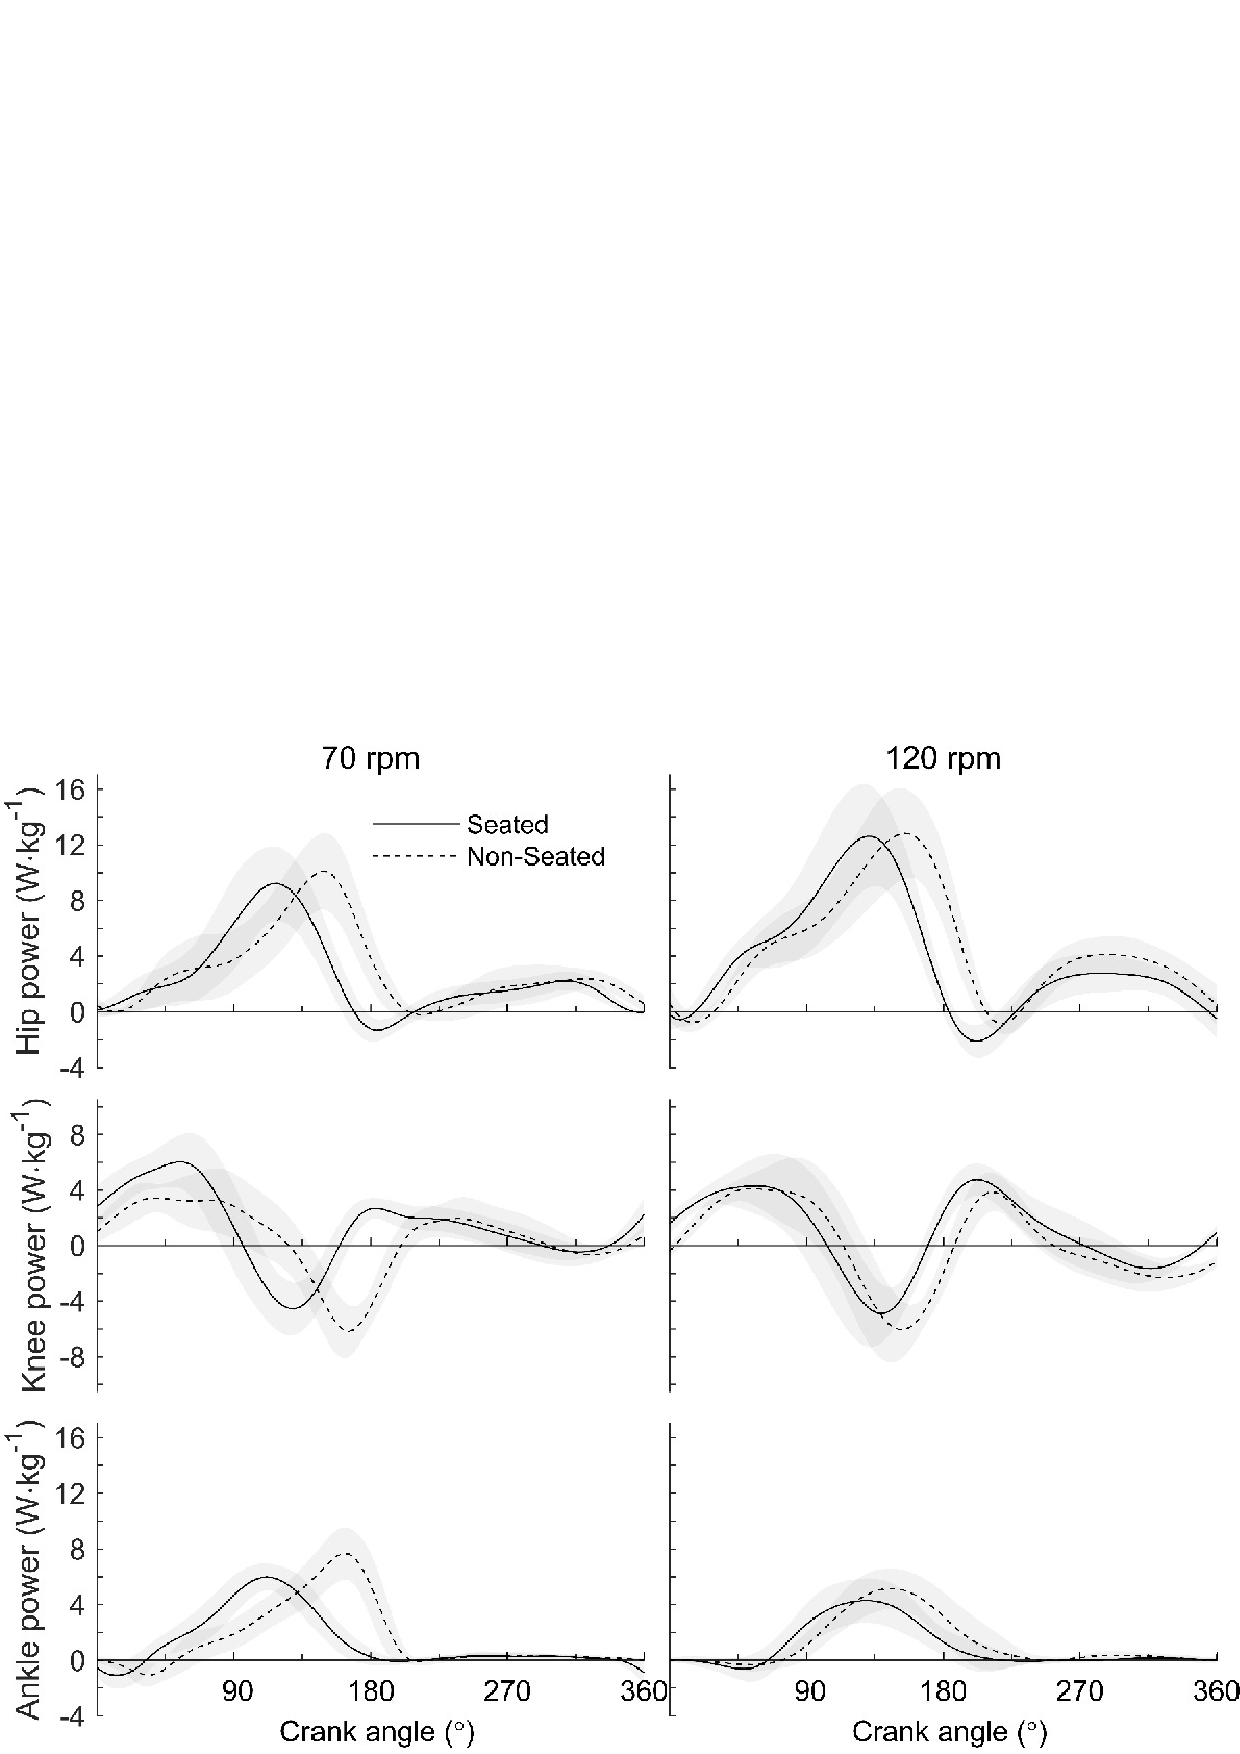
\includegraphics[width=\textwidth]{Study2/Figure2.png}
    \caption[Changes in kinetic energy of the rider's CoM had little impact on the overall total mechanical energy changes.]{\textbf{Changes in kinetic energy of the rider's CoM had little impact on the overall total mechanical energy changes.} Group mean mechanical energy changes of the rider's CoM with respect to crank angle (0$^\circ$; top dead centre) during non-seated cycling at a range of power outputs (10$\%$, 30$\%$, and 50$\%$ \textit{P}$_{max.i}$) at 70 rpm (A-C) and 120 rpm (D-F). The changes in energy have been normalised to body mass. The continuous lines in each plot indicate the total mechanical energy \textit{E}$_{tot}$ = \textit{E}$_\textit{P}$ + \textit{E}$_k$. The rate of energy gain and loss by the CoM (i.e. power) can be inferred by the slope of \textit{E}$_{tot}$ in each plot. The dashed lines indicate the gravitational potential energy \textit{E}$_\textit{P}$ = M$_b$gs$_v$ (g = acceleration of gravity, s$_v$ = vertical displacement of the CoM of the body). The dotted lines, indicate the kinetic energy of motion in all axes \textit{E}$_k$ = $\frac{1}{2}$M$_b$v$^2$ (v = resultant velocity of the CoM in x, y and z axes). The changes in kinetic energy had only a small influence on the total change in mechanical energy and were barely distinguishable from zero when generating low crank power at 120 rpm. Note that the total mechanical energy of the CoM is unchanged over the whole crank cycle, therefore only the change in energy is relevant to the quantity of mechanical energy that can be transferred to the crank or stored in elastic structures (i.e. when the change in mechanical energy is below zero) or the amount of work generated by muscle or elastic structures to raise the CoM (i.e. when the change in mechanical energy is above zero).}
    \label{fig:m2f3}
\end{figure}

\begin{figure}[htbp]
    \centering
    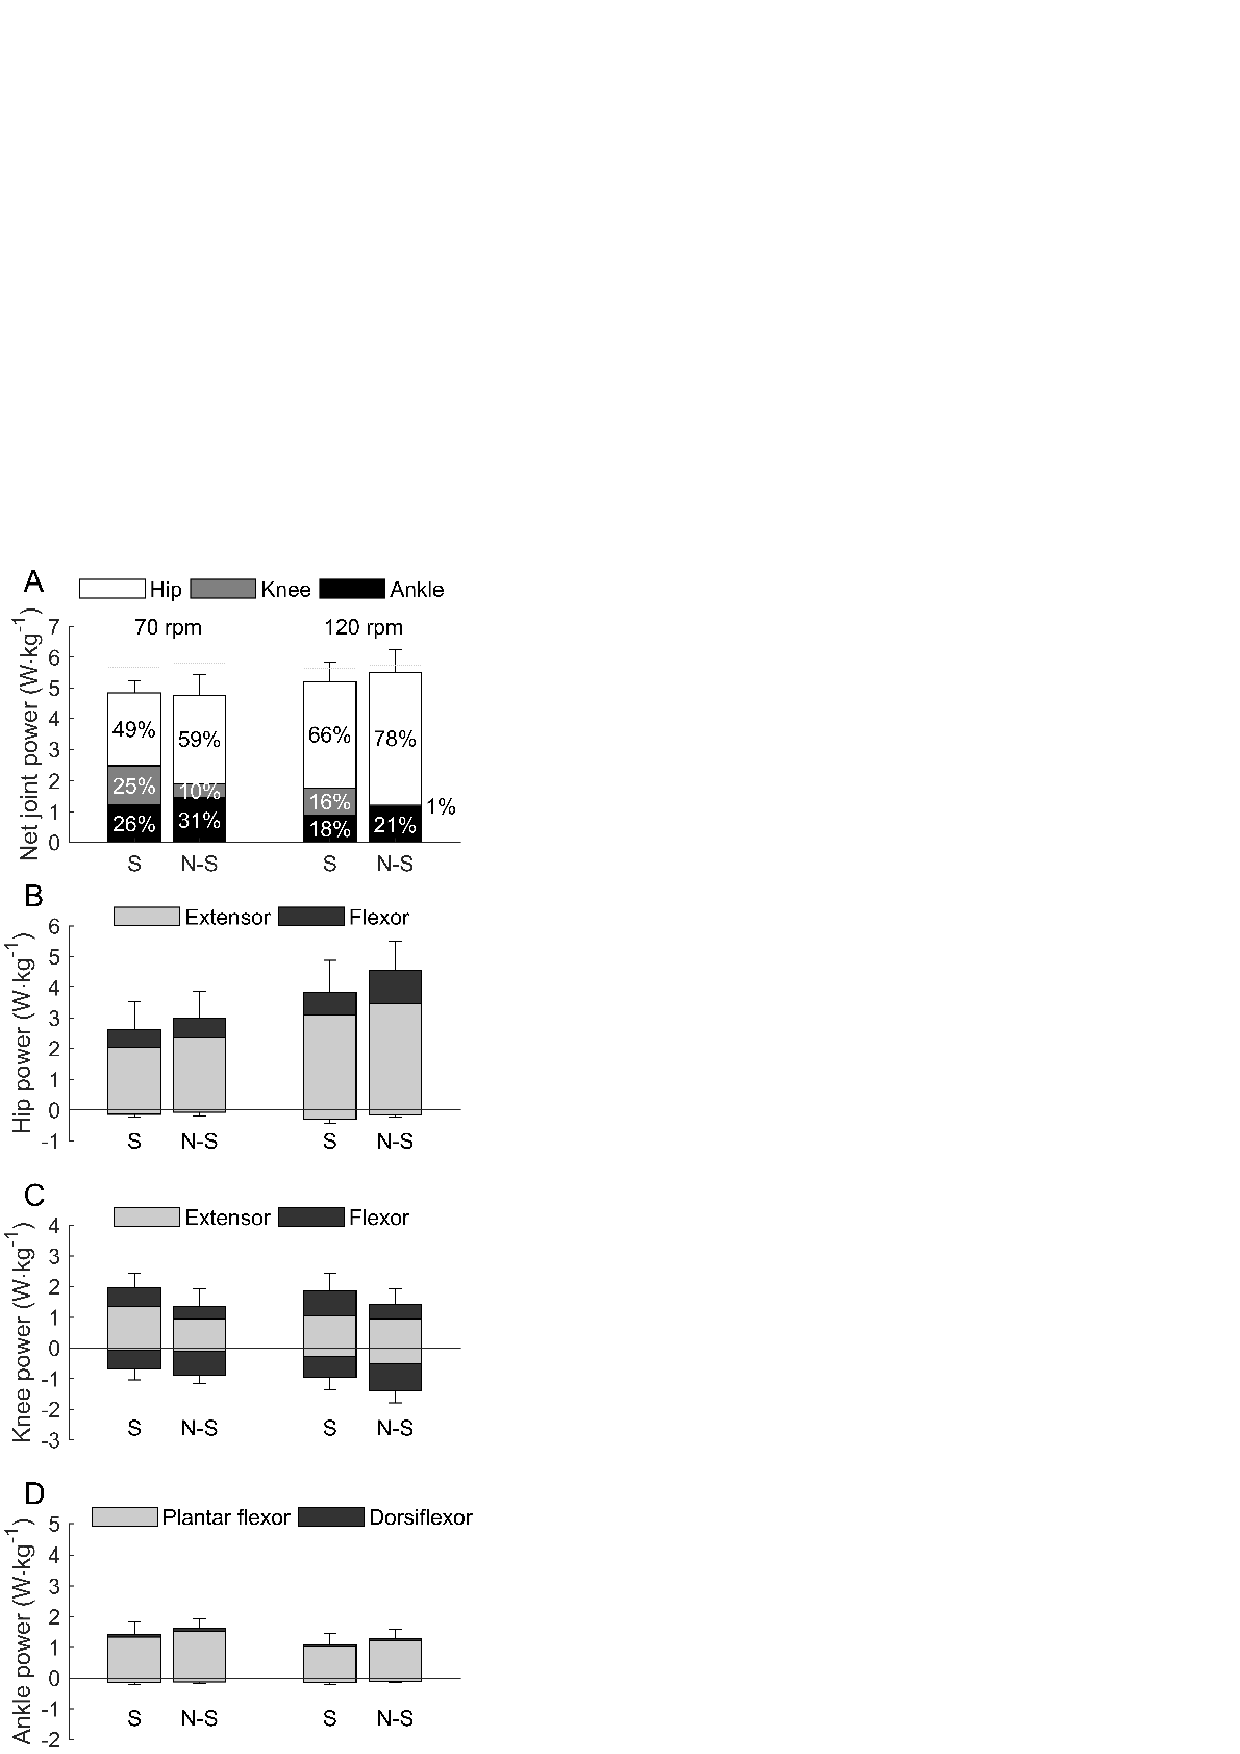
\includegraphics[width=\textwidth]{Study2/Figure3.png}
    \caption[Net upward vertical handlebar forces decrease substantially as power output increases and are much lower at 70 rpm than 120 rpm.especially at 70 rpm.]{\textbf{Net upward vertical handlebar forces decrease substantially as power output increases and are much lower at 70 rpm than 120 rpm.especially at 70 rpm.} Group mean vertical forces during non-seated cycling at a range of power outputs (10$\%$, 30$\%$ and 50$\%$ \textit{P}$_{max.i}$) at 70 rpm (A-C) and 120 rpm (D-F). Forces have been normalised to bodyweight (i.e. M$_b$g = 1; g = acceleration of gravity). F$_{va}$ (continuous lines) indicates the net vertical interaction forces between the bicycle and rider necessary to cause the measured accelerations of the rider's CoM. F$_{vct}$ (dashed lines) indicates the total vertical force at the cranks (F$_{vct}$ = vertical force at right crank + vertical force at left crank). F$_{vhb}$ (dotted lines) indicates the calculated net vertical force acting at the handlebar (F$_{vhb}$ = F$_{va}$ – F$_{vct}$). The mean level of F$_{vhb}$ clearly decreased as power output increased at each cadence. When generating 50$\%$ \textit{P}$_{max.i}$ at 70 rpm, participants generated a net pulling force at the handlebar (i.e. −F$_{vhb}$) during the power phase of each leg, resulting in an 18$\%$ (2.13 $\pm$ 0.75 W$\cdot$kg$^{-1}$) contribution to net crank power by the upper body.}
    \label{fig:m2f4}
\end{figure}

\FloatBarrier

In combination, the phasing and magnitude of changes in \textit{E}$_{tot}$ appear to confirm our final hypothesis that mechanical energy gained by the CoM can be used later in the crank cycle to contribute to positive crank power. Figure 4 shows how mechanical energy lost by the CoM altered the joint power requirements at each instant of the crank cycle. The peak rate of CoM energy loss at each respective power output (10$\%$, 30$\%$, and 50$\%$ \textit{P}$_{max.i}$) was equal to 50$\%$ (2.66$\pm$0.85 W$\cdot$kg$^{-1}$), 25$\%$ (3.50$\pm$0.70 W$\cdot$kg$^{-1}$), and 18$\%$ (3.87$\pm$0.93 W$\cdot$kg$^{-1}$) of peak crank power at 70 rpm; and equal to 26$\%$ (1.21$\pm$0.34 W$\cdot$kg$^{-1}$), 13$\%$ (1.73$\pm$0.78 W$\cdot$kg$^{-1}$), and 13$\%$ (2.88$\pm$1.58 W$\cdot$kg$^{-1}$) at 120 rpm. Although the work performed on the CoM is net zero across a complete crank cycle, the timing of changes in \textit{E}$_{tot}$ dictate whether energy is either absorbed as negative work by muscle, stored as energy in elastic elements, or transferred to the crank. Interestingly, as power output required at the crank increased, the peak rate of CoM energy loss occurred at crank angles closer to horizontal at 70 rpm (10$\%$=134$\pm$11\textdegree, 30$\%$=122$\pm$6\textdegree, 50$\%$=107$\pm$10\textdegree) and 120 rpm (10$\%$=134$\pm$16\textdegree, 30$\%$=131$\pm$14\textdegree, 50$\%$=123$\pm$13\textdegree). These results suggest that the absolute magnitude of power amplification at the crank due to the rate of energy loss by the rider's CoM becomes greater at higher power outputs and at lower cadence.

Additionally, it made conceptual sense that the effects of power output and cadence on changes in \textit{E}$_{tot}$ would be reflected by changes in the pattern of joint power production. Thus, we predicted that changes in power output and cadence would also influence the net power contributed by the lower and upper body. Figure \ref{fig:m2f6} shows the pattern of lower and upper body power production with respect to crank angle in each condition and highlights the simultaneous generation and dissipation of power by the lower and upper body. Figure \ref{fig:m2f7} shows the net contribution of lower and upper body power to total joint power in each condition. The net contribution of upper body power increased with power output under both cadence conditions and was greater at low cadence compared to high cadence. Statistical analysis showed large main effects of power output (\textit{F}=69, $\rho$<0.001, $\eta^2_G$=0.42), cadence (\textit{F}=37, $\rho$<0.001, $\eta^2_G$=0.31), and a moderate interaction effect (\textit{F}=35, $\rho$<0.001, $\eta^2_G$=0.11) on net upper body power. Net upper body power increased significantly with power output at 70 rpm (10$\%$=0.12$\pm$0.26, 30$\%$=1.02$\pm$0.38, and 50$\%$=2.13$\pm$0.75 W$\cdot$kg$^{-1}$) and at 120 rpm (10$\%$=\textminus0.34$\pm$0.67, 30$\%$=0.30$\pm$0.89, and 50$\%$=0.54$\pm$1.02 W$\cdot$kg$^{-1}$) and was significantly greater at 70 rpm than at 120 rpm at each power output. At 70 rpm, the relative contribution of net upper body power to total net joint power increased by 13$\%$, from 5$\%$ at the lowest power output to 18$\%$ at the highest power output. At 120 rpm, the relative contribution of net upper body power to total net joint power was \textminus15$\%$ at the lowest power output and only 5$\%$ at the highest power output. These results provide evidence that muscles in the upper body contribute significant amounts of power to raise the CoM and to generate crank power during non-seated cycling at high power outputs.

\begin{figure}[htbp]
    \centering
    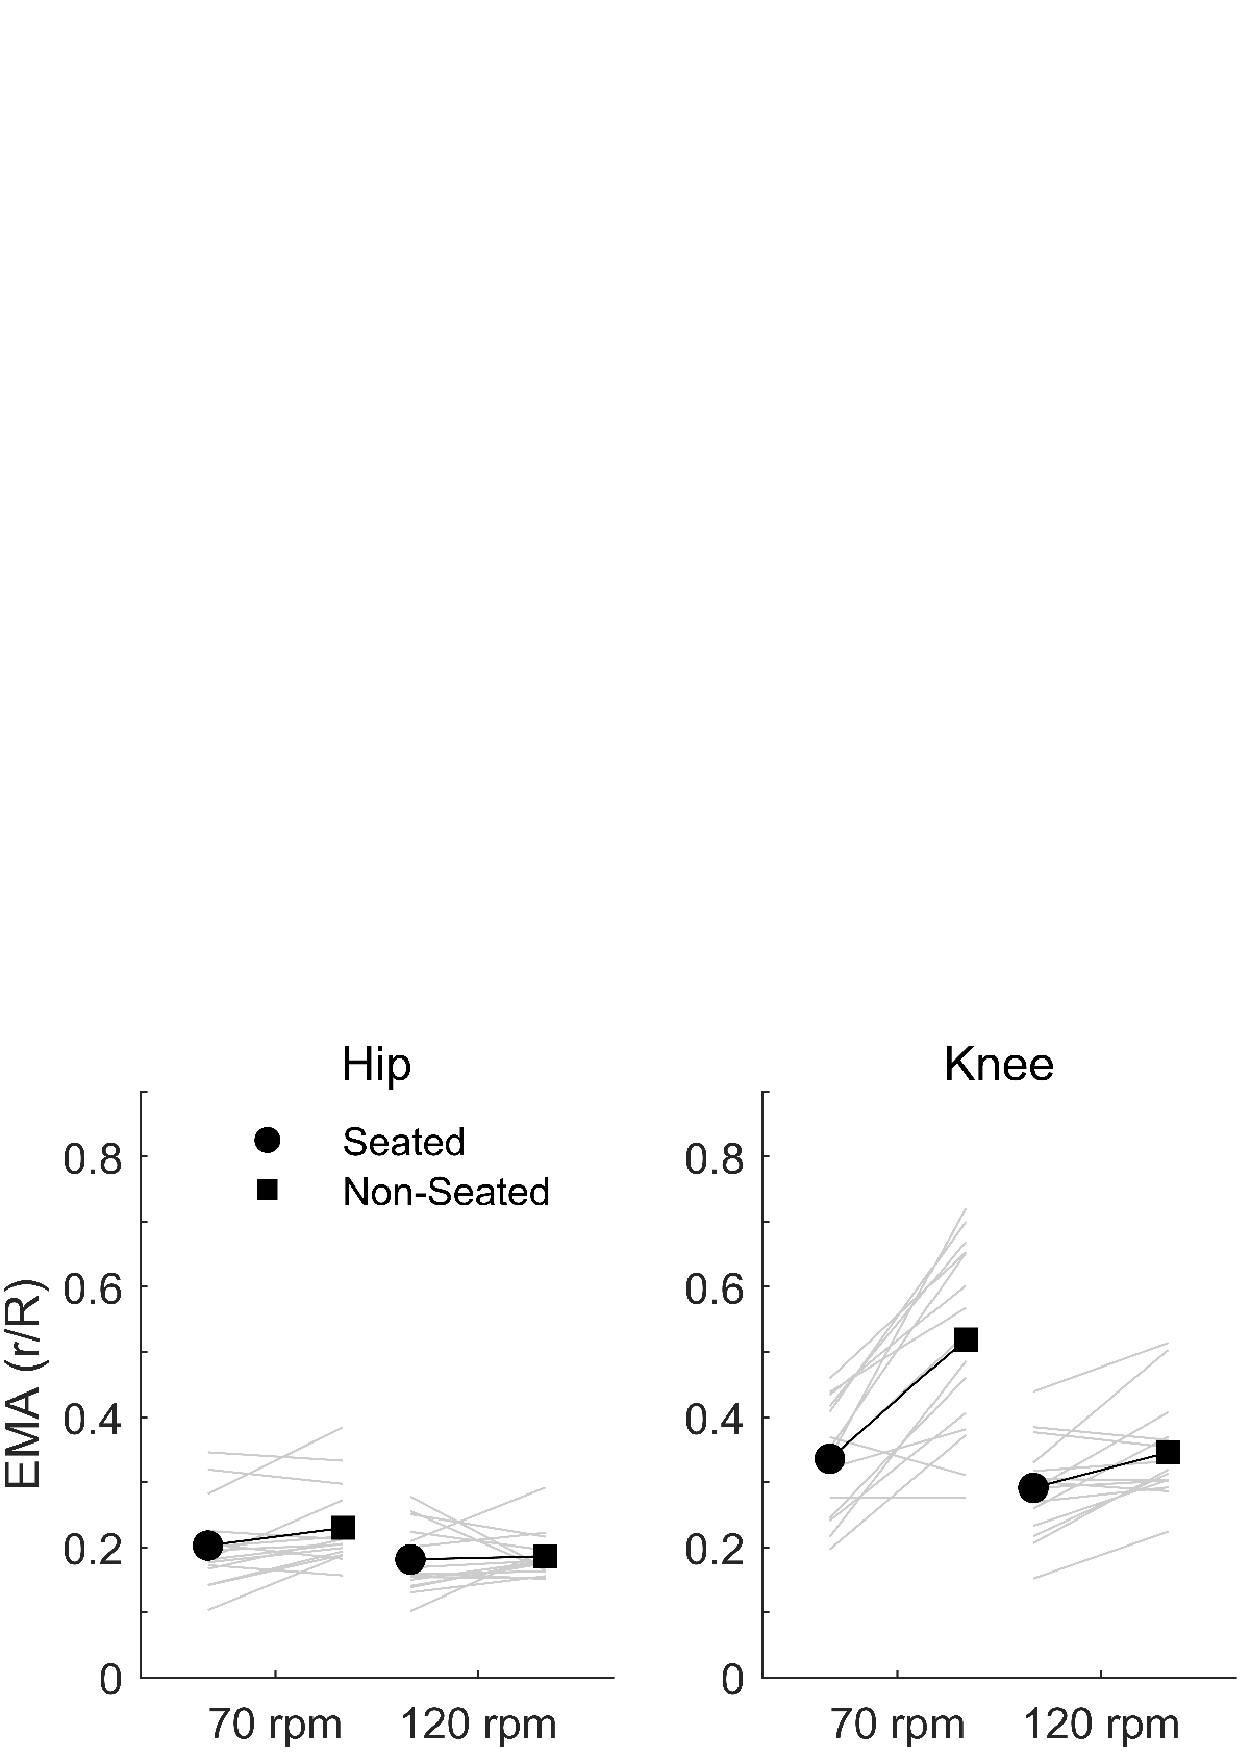
\includegraphics[width=\textwidth]{Study2/Figure4.png}
    \caption[Changes in CoM power are deliberately out of phase with crank power during the period of peak crank power production, meaning that peak joint power requirements are reduced.]{\textbf{Changes in CoM power are deliberately out of phase with crank power during the period of peak crank power production, meaning that peak joint power requirements are reduced.} Group mean total joint power generated by the rider normalised to body mass (\textit{P}$_{tot}$, continuous line) separated into the measured power at both cranks (\textit{P}$_{cranks}$, dashed line) and the rate of energy gained and lost by the rider's CoM (\textit{P}$_{CoM}$, dotted line) over a complete a crank cycle during non-seated cycling at each power output (10$\%$, 30$\%$, and 50$\%$ \textit{P}$_{max.i}$) at 70 rpm (A-C) and 120 rpm (D-F). N.B.: Four distinct phases appear during the crank cycle, whereby the CoM is either reducing or increasing the requirement of joint power in relation to crank power. Downward CoM velocity (negative \textit{P}$_{CoM}$) occurs at specific times during the crank cycle to decrease the instantaneous maximal joint power requirement, while power is generated on the CoM during periods of low crank power output.}
    \label{fig:m2f5}
\end{figure}

\begin{figure}[htbp]
    \centering
    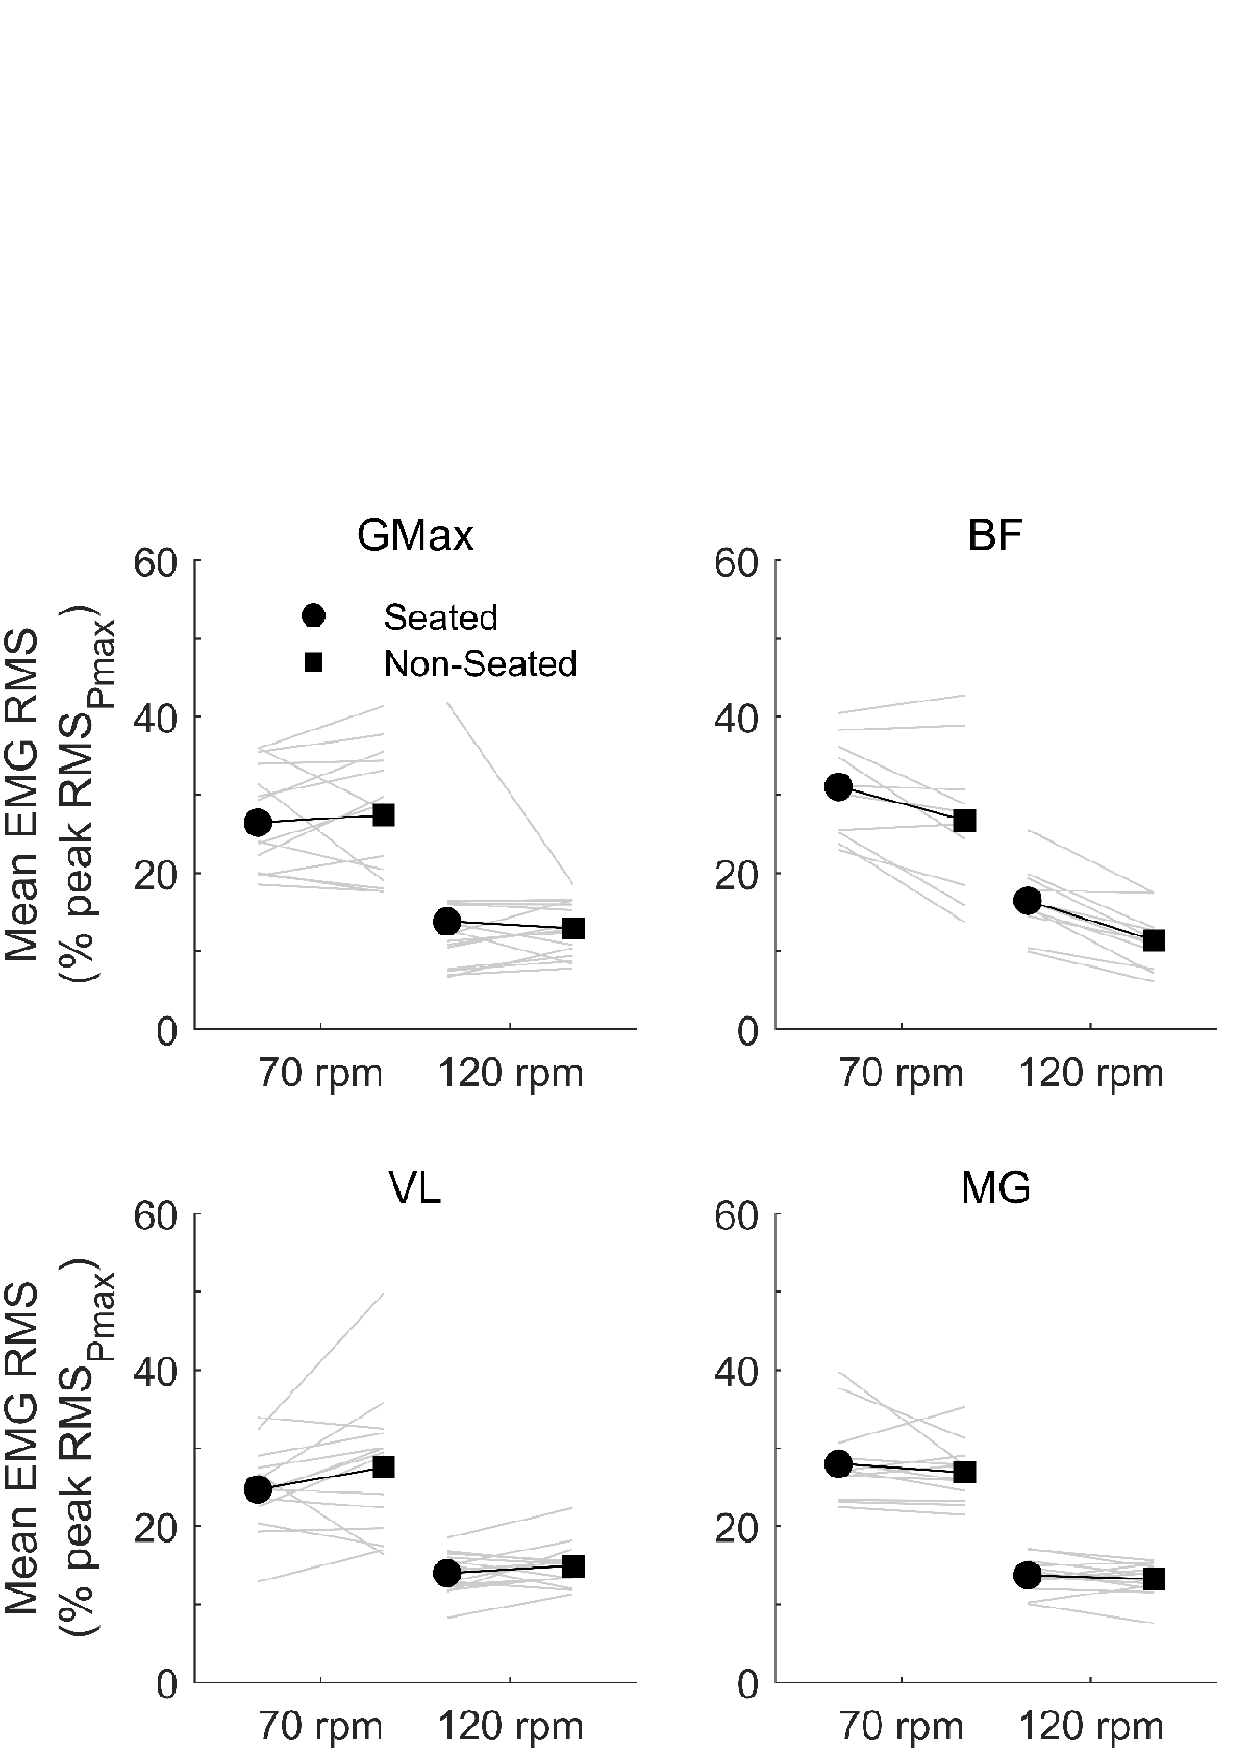
\includegraphics[width=\textwidth]{Study2/Figure5.png}
    \caption[Using a non-seated posture at high cadence resulted in theoretically costly periods of simultaneous power generation and dissipation by the lower body and upper body, respectively.]{\textbf{Using a non-seated posture at high cadence resulted in theoretically costly periods of simultaneous power generation and dissipation by the lower body and upper body, respectively.} Group mean patterns of total joint power output (continuous line) are shown along with the pattern of power production and absorption by the lower body (dashed line) and upper body (dotted line) during non-seated cycling at each power output (10$\%$, 30$\%$ and 50$\%$ \textit{P}$_{max.i}$) at 70 rpm (A-C) and 120 rpm (D-F). N.B.: The upper body generates power in all conditions, but simultaneously absorbs greater amounts of power while the legs are generating power at 120 rpm. These results point towards the inefficiency of having to support bodyweight in the non-seated posture under conditions of lower power and high cadence.}
    \label{fig:m2f6}
\end{figure}

\begin{figure}
    \centering
    \includegraphics[width=\textwidth]{Study2/Figure6.png}
    \caption[Riders use their upper body to contribute greater amounts of power as power output increases.]{\textbf{Riders use their upper body to contribute greater amounts of power as power output increases.} Group mean net power contributions of the lower (\textit{P}$_{lb}$) and upper body (\textit{P}$_{ub}$) to total power output (\textit{P}$_{tot}$) during non-seated cycling at each power output (10$\%$, 30$\%$ and 50$\%$ \textit{P}$_{max.i}$) and cadence (70 rpm and 120 rpm). Power has been normalised to body mass (kg). Pub at each respective power output (10$\%$, 30$\%$ and 50$\%$ \textit{P}$_{max.i}$) was equal to 5$\%$ (0.12$\pm$0.25 W$\cdot$kg$^{-1}$), 14$\%$ (1.00$\pm$0.38 W$\cdot$kg$^{-1}$), and 18$\%$ (2.09$\pm$0.73 W$\cdot$kg$^{-1}$) of total power output at 70 rpm and equal to \textminus15$\%$ (\textminus0.34$\pm$0.66 W$\cdot$kg$^{-1}$), 4$\%$ (0.29$\pm$0.88 W$\cdot$kg$^{-1}$), and 5$\%$ (0.54$\pm$1.00 W$\cdot$kg$^{-1}$) at 120 rpm. The contribution of upper body power increases roughly linearly as total power output requirements increase, with a seemingly steeper increase at 70 rpm.}
    \label{fig:m2f7}
\end{figure}

\FloatBarrier
\section{Discussion}
Our results confirmed that significant vertical oscillations of the rider's CoM occurred during non-seated cycling and caused equivalently scaled oscillations in total CoM mechanical energy. Greater amounts of energy were gained and lost by the CoM at higher power outputs and when cadence was decreased. This increase was a result of an increase in the time over which forces above bodyweight were applied to the CoM. When people are able to freely choose their motion during cycling on an ergometer, power generated by muscle was required to raise the CoM to increase its potential energy, while energy lost by the CoM was due to an exchange of energy with the crank. In all but the low power, fast cadence condition (10$\%$ \textit{P}$_{max.i}$ at 120 rpm), potential energy gained by the CoM was used in the crank cycle to decrease the peak instantaneous joint power requirements. These results provide preliminary mechanical evidence that inertia forces due to vertical acceleration of the CoM can help riders achieve crank forces greater than bodyweight, which adds to the existing body of evidence pertaining to the benefits of foregoing bodyweight support at the saddle when trying to sustain or produce near maximal power outputs \autocite{Stone1993,Caldwell1998,ReiserII2002,Hansen2008,Turpin2016,Soden1978,Costes2015,Hug2011}. 

Work generated by muscle raised the potential energy of the CoM, which was used later in the crank cycle to reduce the peak instantaneous joint power requirement. We know that muscles are both force and power limited \autocite{Galantis2003}, and high forces combined with high shortening velocities  must require higher activations \autocite{Lichtwark2005}. Different muscle fiber types also differ in the energy required to produce a unit of force \autocite{Sargeant2007}. Thus, reducing the peak joint power required during each crank cycle is likely to help riders maintain high-power outputs for a longer duration. Previous research supports this theory, showing that riders use a non-seated posture to increase time to exhaustion at high-power outputs \autocite{Hansen2008}. We also predict that CoM vertical movement during non-seated cycling can be a strategy for increasing \textit{P}$_{max.i}$. 

Our findings agree with earlier cycling research, showing that the upper body joint power contributes significantly to crank power output \autocite{Baker2002}. Greater upper body joint power contributions occurred at higher power outputs and when cadence was reduced, helping to explain why maximal power outputs are higher when riders are able to grip the handlebar \autocite{Baker2002} and, theoretically, that greater levels of crank torque could also be achieved. Force produced at the handlebar is crucial for first raising the potential energy of the CoM and then acting in the opposite direction to give the CoM downward momentum prior to when peak forces are required. As supported by previous literature \autocite{Stone1993}, the arms play an active role to ensure that lower body power contributes to crank power rather than raising the CoM against gravity. For example, maximal power output produced over one crank cycle during seated cycling is reduced by 22$\%$ when riders are not able to grip the handlebar \autocite{Baker2002}. We suspect that in this scenario, the lower limbs produce the same level of power as when gripping the handlebar, but a portion of power is lost due to no contribution of upper body muscle power and an additional portion of power is lost due to the lower limbs generating power on the CoM rather than the crank.

We can only speculate that riders may store energy in passive elastic elements of muscle during non-seated cycling. Theoretically, almost no additional energy would be required to lift the CoM if the decrements in \textit{E}$_{tot}$ could be stored in muscle's elastic elements and then re-used during a later part of the crank cycle. It seems, however, that this scenario does not occur, or is minor, as the majority of \textit{E}$_{tot}$ is transferred to the crank. Further research is required at a muscle level to determine whether there is any potential for energy not transferred to the crank to be stored as elastic energy. 

It is generally accepted that the metabolic cost of positive muscular work is roughly four times that of its mechanical output \autocite{Margaria1968}. For this reason, one may theorize that the muscular work used to raise the CoM is either performed by choice or perhaps cannot be avoided. Here we have provided evidence for the former, showing that the magnitude and phasing of CoM mechanical energy changes can contribute to net positive power at the crank. If the goal of the rider is to minimise energy expenditure, then the cost of supporting extra bodyweight and producing work on the CoM must be considered against the rate and amount of mechanical energy that can be transferred between the CoM and the crank. In this regard, recent findings \autocite{Wilkinson2020a} suggest that riders may be able to partially offset the cost of supporting extra bodyweight in the non-seated posture by increasing effective mechanical advantage at the knee. While metabolic cost is important to the rider during steady-state cycling, it is of no concern when they are attempting to produce maximal power output i.e. during a finishing sprint. Thus, raising and lowering the CoM appears to provide a potential performance advantage to the rider during short-lasting very-high-power output cycling.

Our findings are valid only for cycling on a stationary ergometer whereby the lateral dynamics of the bicycle are constrained. Under normal cycling conditions, particularly during climbing and sprinting, the bicycle leans from side to side during each crank cycle. Although this motion occurs about the bicycle's roll axis, it may have a significant impact on gravitational potential energy changes of the rider's CoM and joint power production. The bicycle's CoM will also rise and fall as the bicycle leans from side-to-side. Although these changes are likely small due to the low mass of the bicycle, it is possible that bicycle and rider CoM mechanical energy changes may be in- or out-of-phase, which potentially impacts on mechanical energy changes of the system. Thus, there is a need for further analyses of rider kinematics and joint mechanics under conditions where lateral bicycle dynamics are unconstrained.

This study is the first to measure rider CoM movement and the associated mechanical energy changes during non-seated cycling. Mechanical energy fluctuations of the rider's CoM are primarily due to changes in gravitational potential energy during the crank cycle. These results show that riders can utilise their body mass to significantly amplify instantaneous maximal crank power output when cycling in a non-seated posture. Under the conditions tested here, this mechanism of power amplification significantly reduced peak joint power requirements, which may underlie why using a non-seated posture can increase time to exhaustion when cycling at high power outputs. It is also possible that raising and lowering the CoM to amplify crank power underlies previous findings that maximal crank power output is higher in the non-seated posture compared to when seated. Our future focus will be to investigate whether similar CoM mechanical energy changes occur when cycling in a non-seated posture under field conditions. The trade-off between the benefits of CoM mechanical energy changes and the separate costs of supporting bodyweight, producing work on the CoM, and potential increase in frontal surface area should also be investigated.